\chapter{绪论}

\section{流变学介绍}
\subsection{流变学的核心研究内容}
流变学是研究物质在外力作用下变形和流动的科学,其研究对象涵盖了流体、软固体以及在特定条件下可以流动的固体\cite{dealyIntroductionRheology1990}。流变学的核心在于揭示材料的应力、应变和时间之间的内在关系,并通过本构方程(流变状态方程)对这些关系进行定量描述。流变学的研究不仅深化了对材料力学行为的理解,还为工程应用和科学研究提供了重要的理论基础。流变学的核心研究内容主要包括以下几个方面\cite{elleroTanner90Years2024,ewoldtDesigningComplexFluids2022}:
\begin{enumerate}[topsep = 0 pt, itemsep= 0 pt, parsep=0pt, partopsep=0pt, leftmargin=44pt, itemindent=0pt, labelsep=6pt, label=(\arabic*)]
  \item 材料的流动与变形行为:材料的流动与变形行为是流变学研究的核心内容之一。通过实验和理论模型,流变学揭示了材料在外力作用下的复杂力学行为。例如,蠕变现象(即在恒定应力下,材料的变形随时间逐渐增加)和应力松弛现象(即在恒定应变下,材料的应力随时间逐渐减小)是流变学中重要的研究对象\cite{BARNES19971,banerjeeRoleRheologyMorphology2023}。这些现象不仅反映了材料的时间依赖性行为,还为材料的长期性能评估提供了理论依据。此外,流变学还研究了材料的非线性力学行为,如屈服、塑性变形和断裂等,这些研究对于理解材料的宏观力学性能具有重要意义\cite{zenerElasticityAnelasticityMetals1949,hajikarimiViscoelasticityTheoreticalBackground2023}。
  \item	  本构方程的构建:本构方程是流变学中用于描述材料力学行为的数学工具,其核心在于建立应力、应变和时间之间的定量关系。对于牛顿流体,其本构方程基于牛顿黏性定律,即应力与应变率成正比\cite{elleroTanner90Years2024}。然而,对于非牛顿流体和软固体,其本构方程则更为复杂,通常需要考虑材料的非线性、黏弹性以及时间依赖性等特性\cite{sunReviewConstitutiveModels2024}。通过构建合理的本构方程,流变学能够对各种物理现象进行精确的数学描述,从而为工程设计和材料开发提供理论支持。
  \item  实验与模拟方法:流变学实验是研究材料流变性能的重要手段,常见的实验方法包括蠕变实验、应力松弛实验和动力试验等\cite{ewoldtDesigningComplexFluids2022}。这些实验能够直接测量材料在不同条件下的力学响应,为理论模型的验证和优化提供实验数据。近年来,随着计算模拟技术的发展,流变学研究逐渐从唯象模型向定量科学转变。微观实验技术(如X射线散射、中子散射)与计算模拟的结合,使得研究者能够在微观尺度上揭示材料的流变机制,从而推动流变学向更高精度和更深层次发展\cite{kuschelNonlinearEnhancementUltrafast2025,sun2022relaxation}。
\end{enumerate}
\subsection{流变学研究及应用方向}
流变学的研究方向广泛,涵盖了多个学科和领域,例如高分子流变学研究高分子材料的分子结构与其流变行为的关系,例如聚合物熔体和溶液的拉伸流变行为\cite{lingComparisonReviewClassical2023}。生物流变学研究生物材料(如血液、肌肉)的流变特性,揭示生理和病理过程中的力学机制\cite{martin2023rheology,jeon2023review}。地质流变学研究岩石、土壤等地质材料的流变行为,应用于地震预测、矿产资源开发等领域\cite{campbellNewtonianPowerLaw2018}。工业流变学在材料加工\cite{banerjeeRoleRheologyMorphology2023}、食品工业\cite{schreuders2022non}、化妆品和医药制造等领域\cite{kim2024role,murch2024non},流变学用于优化工艺和产品性能\cite{zhangModificationTechnologiesConstitutive2024}。非牛顿流体力学研究不符合牛顿黏性定律的流体(如油漆、泥浆、血液)的流动特性\cite{sunReviewConstitutiveModels2024,wang2023non,lowe2019rheology}。

\section{本构方程}
\subsection{线性本构方程}
凝聚相物质分为固体或液体,固体和液体之间的一个区别特征是它们对施加的力的响应。固体在变形时储存能量,如果变形很小,则在消除力后会恢复到原来的形状。相比之下,液体则会通过耗散能量和调整其形状来抵抗力\cite{ricarteTutorialReviewLinear2024,yaoInelasticFluidModels2024}。这种区别可以通过两种经典的力学模型来描述:胡克固体(Hookean Solid) 和牛顿流体(Newtonian Fluid)。胡克定律(Hooke's Law)可以来描述小变形下的弹性固体行为。胡克定律表明,固体的应力$\sigma$与应变$\gamma$成正比,如公式\eqref{eq:hookean_solid}所示。其中,$G$为弹性模量,用于描述材料在弹性变形范围内抵抗外力的能力。它反映了材料的刚度,即材料在受力时发生变形的难易程度。弹性模量越大,材料越难变形;弹性模量越小,材料越容易变形。胡克固体是理想化的弹性固体模型,适用于描述金属、陶瓷等材料在小变形条件下的力学行为\cite{sunReviewConstitutiveModels2024}。
\begin{equation}
  \sigma = G \gamma  \label{eq:hookean_solid}
\end{equation}
而对于液体,其对外力的响应则完全不同。液体无法储存能量以恢复形状,而是通过内部的粘性阻力来耗散能量,并持续流动以适应外力。这种行为可以用牛顿流体的本构方程来描述,即剪切应力与剪切速率成正比,如公式\eqref{eq:newton_fluid}所示。其中,$\eta$为粘性系数,用于描述液体在运动过程中耗散能量的能力。粘性系数越大,液体越容易耗散能量,反之亦然。牛顿流体是理想化的粘性流体模型,适用于描述水、空气等液体在运动过程中耗散能量的行为\cite{ricarteTutorialReviewLinear2024}。
\begin{equation}
  \sigma = \eta \dot{\gamma}  \label{eq:newton_fluid}
\end{equation}
然而,这些特征都是理想化的,代表了特定条件的行为。许多凝聚相材料不容易归入这些经典类别,因为它们的机械性能取决于变形的大小、速率、变形历史,加载过程等等。例如,考虑牙膏,它像液体一样流动,可以将其从管中挤出,但一旦放在牙刷上,它就会像固体一样保持其形状。这类物质同时具有黏性和弹性,被认为是黏弹性材料,被称为软物质或者复杂流体\cite{songNonMaxwellianViscoelasticStress2023}。

线性黏弹性理论认为在小变形范围(线性范围内)应力-应变关系是线性的,即应力与应变成正比。同时线性黏弹性区间内材料具有时间依赖性,材料的力学响应不仅取决于当前的应力或应变,还依赖于时间或加载历史。
\begin{figure}[htbp]
  \centering
  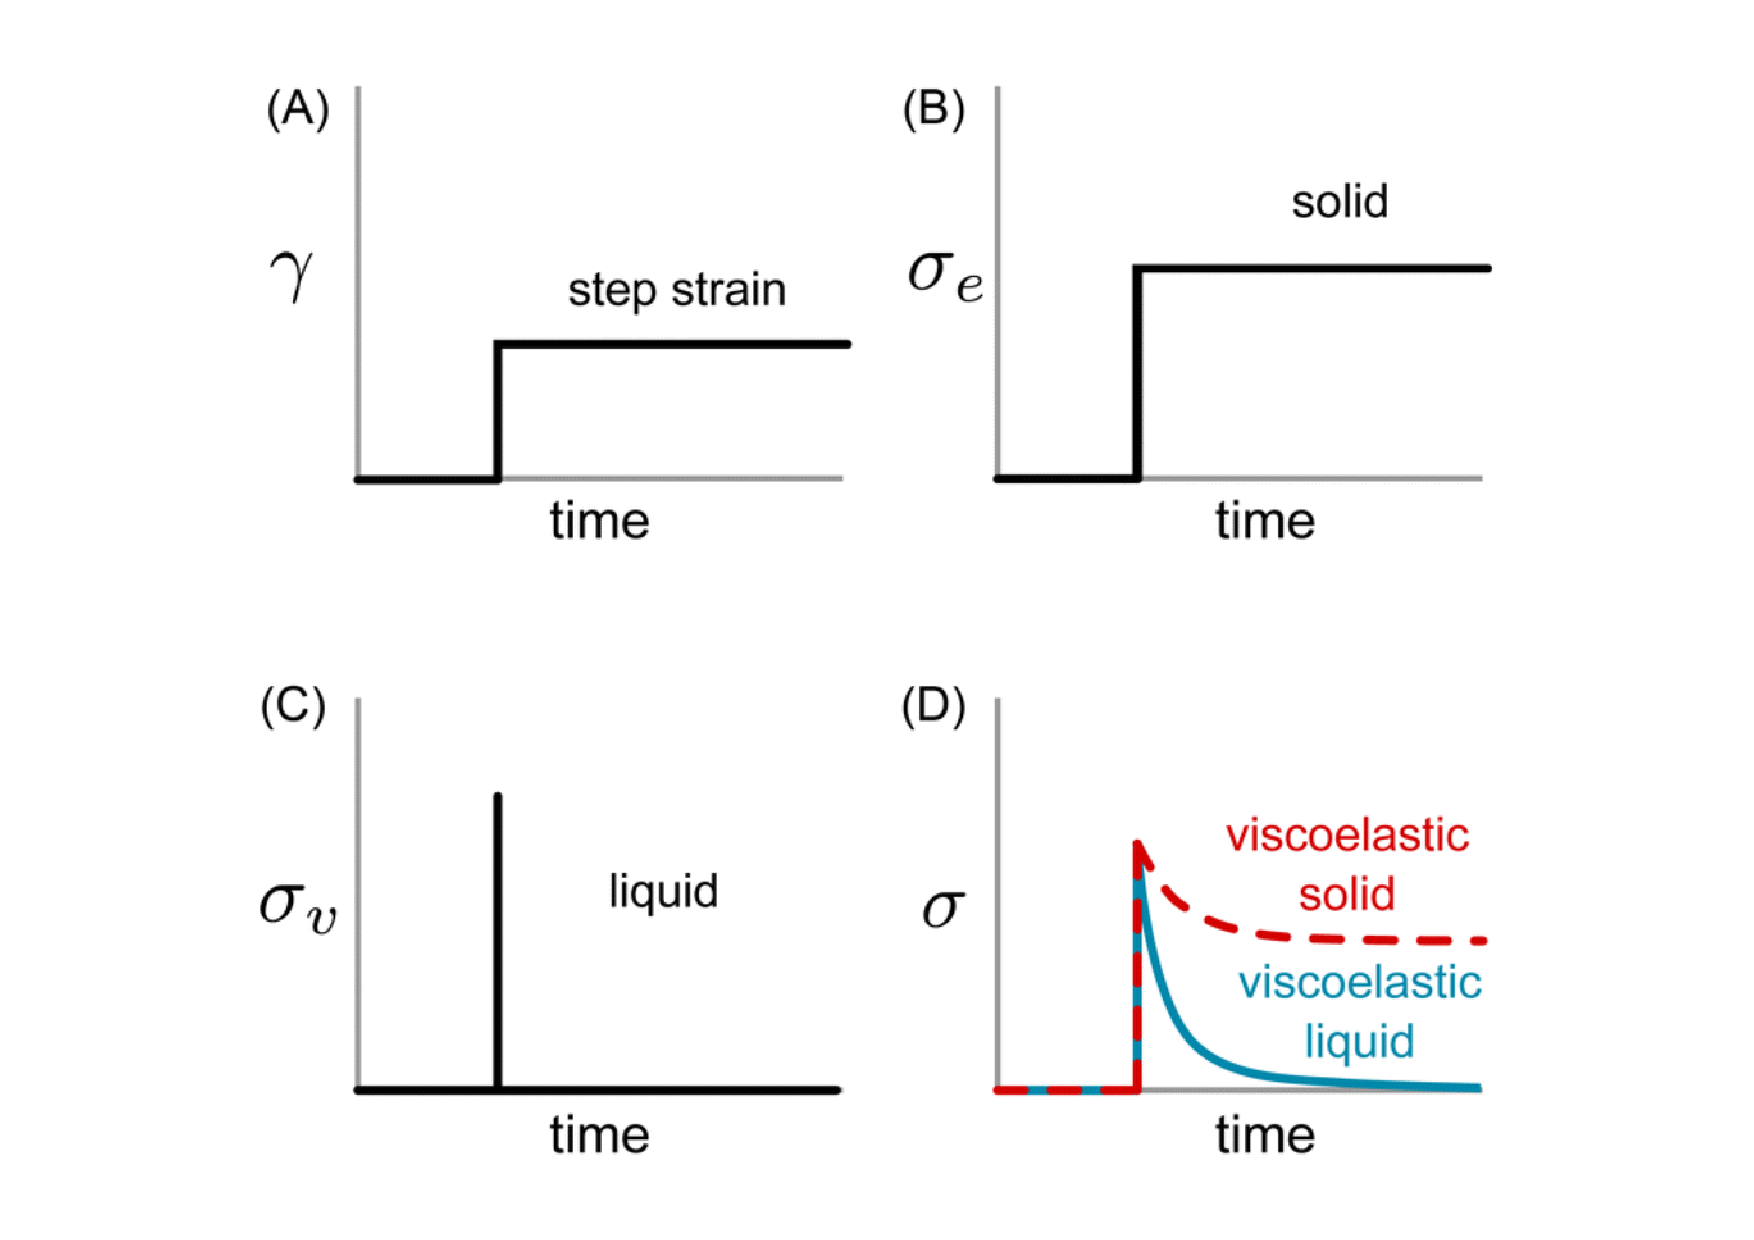
\includegraphics[width=\textwidth]{Fig/solid_liquid.pdf}
  \FigureBicaption{\label{differ_fluid_intro}(A)施加的应变曲线以及对应的剪切应力(B)理想弹性固体(C)理想粘性液体(D)粘弹性样品\cite{ricarteTutorialReviewLinear2024}}{(A) Applied strain profile and resulting shear stress (B) Ideal elastic solid (C)Ideal viscous liquid (D) Viscoelastic samples\cite{ricarteTutorialReviewLinear2024}}
\end{figure}
图\ref{differ_fluid_intro}概述了两种不同类型的粘弹性材料的简单剪切行为。对于粘弹性固体和液体,阶跃应变会引起瞬时弹性响应,从而产生$\sigma$峰值。然而,应力不是保持不变或立即降至零,而是逐渐降低。它在很长一段时间内接近粘弹性固体的有限平台值,而粘弹性液体则完全衰减到零\cite{ricarteTutorialReviewLinear2024}。

线性本构理论中最经典的是Maxwell模型\cite{maxwell1867iv},如图\ref{maxwell_intro}所示,Maxwell模型将材料的弹性行为和粘性行为结合起来,它用一个弹簧(弹性元件)和一个粘壶(粘性元件)串联表示黏弹性关系。Maxwell模型的微分形式如公式\eqref{eq:maxwell_model_dt}所示,其中$\tau$表示松弛时间,等于$eta/G$。将两边积分得到Maxwell模型的积分形式如公式\eqref{eq:maxwell_model_int}所示。
\begin{align}
   & \frac{d\sigma}{dt} + \frac{\sigma}{\tau}  = G \frac{d\gamma}{dt} \label{eq:maxwell_model_dt}                                                   \\
   & \sigma(t)                                = \int_{-\infty}^{t} G e^{-\frac{t-t'}{\tau}} \frac{d\gamma(t')}{dt'} dt'\label{eq:maxwell_model_int}
\end{align}
积分形式的方程显示了任何时刻的应力是松弛模量乘以应变速率的积分,该时刻之前材料的整个历史。由于被积函数中的衰减指数,模型具有衰落的记忆,因此最近的应变历史比过去的应变历史更重要。
\begin{figure}[htbp]
  \centering
  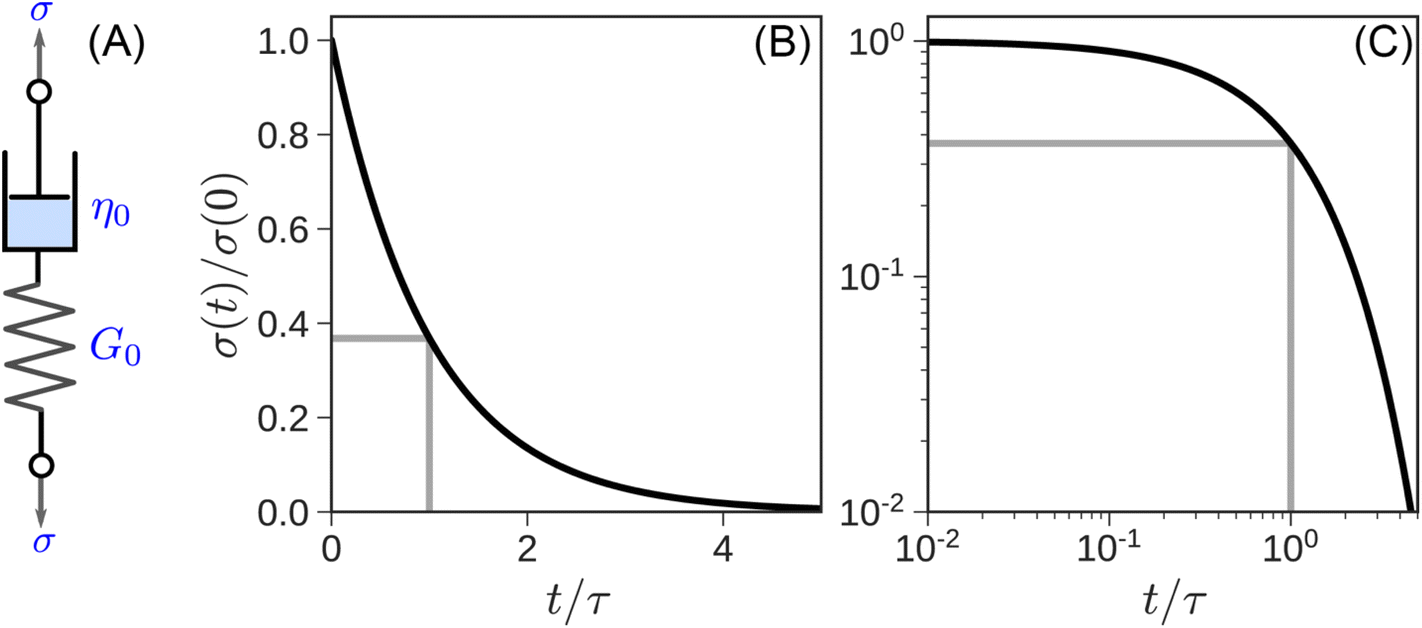
\includegraphics[width=0.8\textwidth]{Fig/maxwell_intro.png}
  \FigureBicaption{\label{maxwell_intro} Maxwell 模型示意图}{Schematic illustration of Maxwell model}
\end{figure}
如果将多个Maxwell模型并联,便可以得到广义Maxwell模型方程,如公式\eqref{eq:generalized_maxwell_model}所示。
\begin{equation}
  \sigma(t) = \int_{-\infty}^{t} G(t-t') \frac{d\gamma(t')}{dt'} dt' \label{eq:generalized_maxwell_model}
\end{equation}
其中松弛模量 \(G(t)\) 定义为公式\eqref{eq:generalized_maxwell_model_G}。
\begin{equation}
  G(t) = \sum_{i=1}^{n} G_i e^{-\frac{t}{\tau_i}} \label{eq:generalized_maxwell_model_G}
\end{equation}

Maxwell模型通过将黏弹性抽象为黏性元件和弹性元件串联来得到本构方程。如果将弹簧和粘壶进行并联,则得到Kelvin-Voigt模型的本构方程,即公式\eqref{eq:kelvin_voigt_model}\cite{voigt1892ueber}。
\begin{equation}
  \sigma(t) = G \gamma(t) + \eta \frac{d\gamma(t)}{dt} \label{eq:kelvin_voigt_model}
\end{equation}
将多个Kelvin-Voigt模型的元件进行串联,便可以得到广义Kelvin-Voigt模型,如公式\eqref{eq:generalized_kelvin_voigt_model}。
\begin{equation}
  \sigma(t) = \sum_{i=1}^{n} \left( G_i \gamma_i(t) + \eta_i \frac{d\gamma_i(t)}{dt} \right)\label{eq:generalized_kelvin_voigt_model}
\end{equation}
原则上,任何广义Voigt模型都可以在数值上映射到等效的广义 Maxwell模型,这是线性本构方程构建的基本研究方法的不同角度\cite{ricarteTutorialReviewLinear2024}。

如果将传统的整数阶导数模型改为分数阶导数,能够更加准确描述材料的记忆效应。例如Bagley和Torvik等在20世纪80年代提出的分数阶Maxwell模型,是对传统Maxwell模型的推广\cite{bagley1986fractional}。无论是什么形式的线性本构方程,均满足一个基本假设材料的响应是线性的,即多个应变历史的叠加效应等于各自效应的线性相加,当公式\eqref{eq:generalized_maxwell_model}中的松弛模量G表示为公式\eqref{eq:generalized_maxwell_model_G}时是Maxwell模型的形式,事实上当G为一个抽象的松弛函数时,公式\eqref{eq:generalized_maxwell_model}抽象为更一般的线性本构方程,被称为玻尔兹曼叠加原理(BSP),玻尔兹曼叠加原理广泛应用于描述线性黏弹性材料的行为,例如应力松弛、蠕变、动态力学响应等\cite{boltzmannZurTheorieElastischen1878}。
\subsection{非线性本构方程}
线性本构方程只能用于描述只能描述简单的材料行为,例如弹性变形、小应变下的黏弹性行为\cite{fedorowiczElasticPerfectlyPlastic2024,lingComparisonReviewClassical2023,ricarteTutorialReviewLinear2024}。适用于材料在小变形范围内的线性响应。能够描述复杂的材料行为,而非线性本构方程可以用来描述更为复杂的行为例如塑性变形、硬化或软化、各向异性、大变形、剪切稀化、剪切增稠等行为。绝大部分高分子材料具有较复杂的非线性关系。Binham提出模型认为屈服性流体当剪应力低于屈服应力时,流体表现为刚性固体;当剪应力超过屈服应力时,流体开始流动,且流动行为类似于牛顿流体\cite{binghaminvestigation}。Herschel-Bulkley模型在此基础之上引入了剪切稀化和剪切增稠的表示,如公式\eqref{eq:herschel},是描述非线性本构方程的一套公式\cite{herschel1926konsistenzmessungen}。
\begin{equation}
  \sigma=\sigma_0+K\dot{\gamma}^n \label{eq:herschel}
\end{equation}
松弛模量函数不仅是时间的函数,也是应变的函数,能够表征大变形下的非线性响应。改进的Herschel-Bulkley类模型在Herschel-Bulkley模型的基础上,通过引入额外的参数或修正项,显著提升了对流体行为的描述精度。例如,在Herschel-Bulkley模型中引入高阶项(如剪切速率的二阶项),可以更准确地刻画非线性流变行为\cite{magnon2021precise}。此外,通过引入Papanastasiou正则化方法,有效解决了原始模型在低剪切速率下的数值不稳定性问题,这一改进模型被称为Herschel-Bulkley-Papanastasiou (HBP) 模型。HBP模型在磁流变液等复杂流体的流变特性描述中得到了广泛应用\cite{papanastasiou1987flows}。
Herschel-Bulkley类模型不涉及弹性流体,主要用于解决屈服应力流体的本构问题,对于黏弹性流体的非线性本构方程而言,可以写出一般的通式,如公式\eqref{eq:nolinear_model},非线性黏弹性流体的本构方程主要通过积分和微分形式分别进行描述\cite{ewoldtDesigningComplexFluids2022}。
\begin{equation}
  \sigma(t) = \int_{-\infty}^{t} G(t-t',\gamma) \frac{d\gamma(t')}{dt'} dt' \label{eq:nolinear_model}
\end{equation}

微分形式的Oldroyd-B模型,如公式\eqref{eq:oldroyd_b}是在Maxwell模型的基础上作了修正,增加了延迟时间项$\lambda_2$ ,从而能够描述更复杂的流变行为,同时这个模型引入了上随体导数来代替普通导数,在物理上更加符合真实世界的材料行为\cite{oldroyd1958non}。Oldroyd-B模型本意可以在Weissenberg数($W_i=\lambda_1 \dot{\gamma}_i$)较小的情况下描述线性黏弹性,但是其中的上随体导数在一定程度上包含了部分非线性效应。Oldroyd-B模型是非线性本构方程的经典基础模型,研究者在此基础上为了更准确地描述非线性黏弹性行为,研究者提出了多种修正的 Oldroyd-B模型。
\begin{equation}
  \boldsymbol{\sigma} + \lambda_1 \frac{\mathcal{D}\boldsymbol{\sigma}}{\mathcal{D}t} = \eta \left( \dot{\boldsymbol{\gamma}} + \lambda_2 \frac{\mathcal{D}\dot{\boldsymbol{\gamma}}}{\mathcal{D}t} \right) \label{eq:oldroyd_b}
\end{equation}
Giesekus模型(公式\eqref{eq:giesekus})在Oldryd-B模型基础上,增加了一个非线性项,通过非线性系数$\alpha$来表示非线性行为\cite{giesekus1982simple}。Giesekus模型常用于描述高聚物溶液、熔体以及其他粘弹性流体的流变行为。这些流体通常表现出剪切稀化和弹性效应。尤其是在中等至高剪切速率范围内。其模型参数(如迁移因子α)可以调节剪切稀化的强度和拐点形状,具有较高的灵活性\cite{PENG2021104571,kim2024viscosity}。Giesekus模型在高Weissenberg数(Wi)条件下仍能保持数值稳定性,适用于强弹性效应的流动场景。通过引入对数构象重构等方法,可以进一步提高其在高Wi条件下的计算稳定性\cite{fattal2004constitutive}。
\begin{equation}
  \boldsymbol{\sigma} + \lambda_1 \frac{\mathcal{D}\boldsymbol{\sigma}}{\mathcal{D}t} + \alpha \frac{\lambda_1}{\eta} \boldsymbol{\sigma} \cdot \boldsymbol{\sigma} = \eta \left( \dot{\boldsymbol{\gamma}} + \lambda_2 \frac{\mathcal{D}\dot{\boldsymbol{\gamma}}}{\mathcal{D}t} \right) \label{eq:giesekus}
\end{equation}
PTT模型(公式\eqref{eq:ptt})通过引入一个非线性应力函数$f$扩展了Oldroyd-B模型,该函数通常取指数形式\cite{thien1977new}。
\begin{equation}
  f(\text{tr}(\boldsymbol{\sigma})) \boldsymbol{\sigma} + \lambda_1 \frac{\mathcal{D}\boldsymbol{\sigma}}{\mathcal{D}t} = \eta \left( \dot{\boldsymbol{\gamma}} + \lambda_2 \frac{\mathcal{D}\dot{\boldsymbol{\gamma}}}{\mathcal{D}t} \right) \label{eq:ptt}
\end{equation}
FENE-P模型(公式\eqref{eq:fene_p})在 Oldroyd-B 模型的基础上引入了有限拉伸效应,通过项$\frac{\lambda_1}{\eta} \frac{\boldsymbol{\sigma}}{1 - \text{tr}(\boldsymbol{\sigma})/b}$描述聚合物链的有限拉伸行为\cite{bird1980polymer}。参数$b$表示聚合物链的最大拉伸比。该模型适用于描述聚合物溶液在强流动条件下的非线性行为。
\begin{equation}
  \boldsymbol{\sigma} + \lambda_1 \frac{\mathcal{D}\boldsymbol{\sigma}}{\mathcal{D}t} = \eta \left( \dot{\boldsymbol{\gamma}} + \lambda_2 \frac{\mathcal{D}\dot{\boldsymbol{\gamma}}}{\mathcal{D}t} \right) - \frac{\lambda_1}{\eta} \frac{\boldsymbol{\sigma}}{1 - \text{tr}(\boldsymbol{\sigma})/b} \label{eq:fene_p}
\end{equation}
通过将Oldroyd-B模型与分数阶导数结合,可以得到分数阶Oldroyd-B模型,如公式\eqref{eq:fractional_oldroyd_b}。分数阶 Oldroyd-B模型通过引入分数阶导数描述非局部记忆效应\cite{qi2007stokes}。参数$\alpha$和$\beta$是分数阶导数的阶数,该模型能够捕捉更复杂的流变行为,适用于具有非局部记忆效应的复杂流体。
\begin{equation}
  \boldsymbol{\sigma} + \lambda_1^\alpha \frac{\mathcal{D}^\alpha \boldsymbol{\sigma}}{\mathcal{D}t^\alpha} = \eta \left( \dot{\boldsymbol{\gamma}} + \lambda_2^\beta \frac{\mathcal{D}^\beta \dot{\boldsymbol{\gamma}}}{\mathcal{D}t^\beta} \right) \label{eq:fractional_oldroyd_b}
\end{equation}

另一类本构模型如K-BKZ模型源于积分型Maxwell模型公式\eqref{eq:maxwell_model_int}\cite{kaye1962non,bernstein1963study}。
K-BKZ模型如公式\eqref{eq:k_bkz_model}所示。在 K-BKZ 模型中,$h$ 称为阻尼函数,它是形变张量的第一不变量 $I_1$ 和第二不变量 $I_2$ 的函数。$\mathbf{C}^{-1}(t,t')$ 是Finger 形变张量的逆,用于描述从时间 $t'$ 到 $t$ 的形变历史。$m(t-t')$ 是瞬态函数或记忆函数,用于表征材料对历史形变的记忆效应。K-BKZ模型广泛应用于聚合物加工(如挤出、注塑、热成型等)、生物流体力学(如血液、蛋白质悬浮液等复杂流体的流变行为研究)以及涂料和润滑剂的流动行为和流变特性分析\cite{mitsoulis60YearsKayeBernstein2023}。
\begin{align}
  % K-BKZ 模型基本形式
   & \boldsymbol{\sigma}(t)  = \int_{-\infty}^t m(t-t') \, h(I_1, I_2) \, \mathbf{C}^{-1}(t,t') \, dt'    \label{eq:k_bkz_model}
\end{align}
Doi和Edwards尝试从分子角度构建本构方程,在管子模型的基础上提出了Doi-Edwards模型(公式\eqref{eq:doi_edwards})。Doi-Edwards 模型的核心思想是将高分子链的缠结效应简化为一条光滑管道对链的限制作用,链在管道中的运动通过松弛和扩散来描述\cite{doi1978dynamics1,doi1978dynamics2,doi1978dynamics3,doi1979dynamics4}。其中$G_0$表示松弛时间,而$Q$表示为公式\eqref{eq:doi_edwards_q},反映了高分子链在形变历史下的方向分布变化,即链的取向如何随形变而变化。
\begin{align}
   & \boldsymbol{\sigma}(t)  = G_0 \int_{-\infty}^t \frac{\partial Q(\mathbf{E}(t,t'))}{\partial t'} \, dt'    \label{eq:doi_edwards}                                                                  \\
   & Q(\mathbf{E}(t,t'))     = \frac{5}{2} \left\langle \frac{\mathbf{E}(t,t') \cdot \mathbf{u} \mathbf{u}}{|\mathbf{E}(t,t') \cdot \mathbf{u}|^2} \right\rangle_{\mathbf{u}} \label{eq:doi_edwards_q}
\end{align}
传统的Doi-Edwards模型基于单链平均场近似,将缠结效应简化为一条光滑的“管子”对高分子链的限制作用。然而,这种简化忽略了链-链间的直接相互作用,难以解释快速大形变条件下的非线性流变现象(如应力过冲、缠结点破损和重组等)。近年来,研究者通过引入多链相互作用,提出了修正的管子模型,在此基础之上能够更好地描述缠结高分子流体的非线性行为\cite{OConnor1992ConfirmationOT,hassager2010constitutive,chupin2017mathematical}。

\subsection{传统的本构方程的构建方法}
传统本构方程尤其是Oldroyd-B、Doi-Edwards等复杂的非线性模型具有较多的待定参数,通过数学形式描述材料的应力-应变关系及其对时间、温度和形变历史的依赖性。其构建方法主要基于实验观测、理论推导和数值模拟的结合,通常分为以下几个步骤。

首先,实验观测是构建本构方程的基础。通过流变学实验(如剪切流变、拉伸流变等),研究者可以获取材料在不同形变条件下的应力响应数据。这些实验数据为理论模型的构建提供了关键依据。例如,通过动态力学分析(DMA)测量材料的存储模量和损耗模量,可以确定其粘弹性特性;通过应力松弛和蠕变实验,可以推断材料的记忆效应和时间依赖性。实验数据的精确性和全面性直接决定了本构方程的适用性和预测能力\cite{alvesNumericalMethodsViscoelastic2021,stadlerWhatAreTypical2014}。

其次,对于非线性材料,则需要引入更复杂的本构关系,这里主要还是基于线性黏弹性方程,通过各类引入非线性关系的方法来进行非线性关系推导,理论推导的关键在于如何将微观结构信息(如高分子链的缠结、颗粒的相互作用等)与宏观力学行为联系起来。而对于理论推导的结果,每一个非线性项或参数应当从数学角度进行证明\cite{zhai2024global}。近年来,数学研究者对Doi-Edwards模型的适定性进行了深入研究。Chupin等人通过Schauder不动点定理和Galerkin近似方法,证明Doi-Edwards 模型在二维情况下的全局解存在性和唯一性\cite{hassager2010constitutive}。这一结果为模型的数学基础提供了严格的理论支持。

数值模拟在本构方程的构建和验证中发挥着关键作用。有限元分析(FEA)有限差分法(FDM)和有限体积法(FVM)等数值方法能够将本构方程应用于复杂几何和边界条件下的力学问题,从而模拟材料的应力分布、形变行为和流动特性\cite{alvesNumericalMethodsViscoelastic2021}。分子动力学模拟(MD)是另一种重要的数值工具,能够从分子尺度模拟材料的力学行为,为宏观本构方程的构建提供微观依据。例如,通过粗粒度分子动力学模拟(CGMD),研究者可以研究高分子链的缠结动力学,验证管子模型的假设\cite{li2023coupling,sgouros2017slip}。由于聚合物液体具有单体、中观和宏观流尺度的多尺度特征,因此关联不同层次的多尺度模拟(MSS)能够更准确地再现其流动特性\cite{satoRecentDevelopmentsMultiscale2024}。近年来,基于分子动力学的多尺度模拟方法显著推进了复杂流体本构关系的构建。Webb等人提出基于图论的系统粗粒化方法,通过拓扑约简实现分子结构特征的有效保留,为建立跨尺度本构方程提供了数学基础\cite{webb2018graph}。在此框架下,Behbahani开发了原子模拟-粗粒化-滑移弹簧的分层耦合算法,成功预测了聚乙烯熔体的非线性粘弹性响应\cite{behbahani2021dynamics}。Morii提出的拉格朗日多尺度框架实现了从分子涨落到连续介质流动的全域耦合,在高弹性数工况下展现出优于传统欧拉方法的数值稳定性\cite{morii2021lagrangian}。
\begin{figure}[htbp]
  \centering
  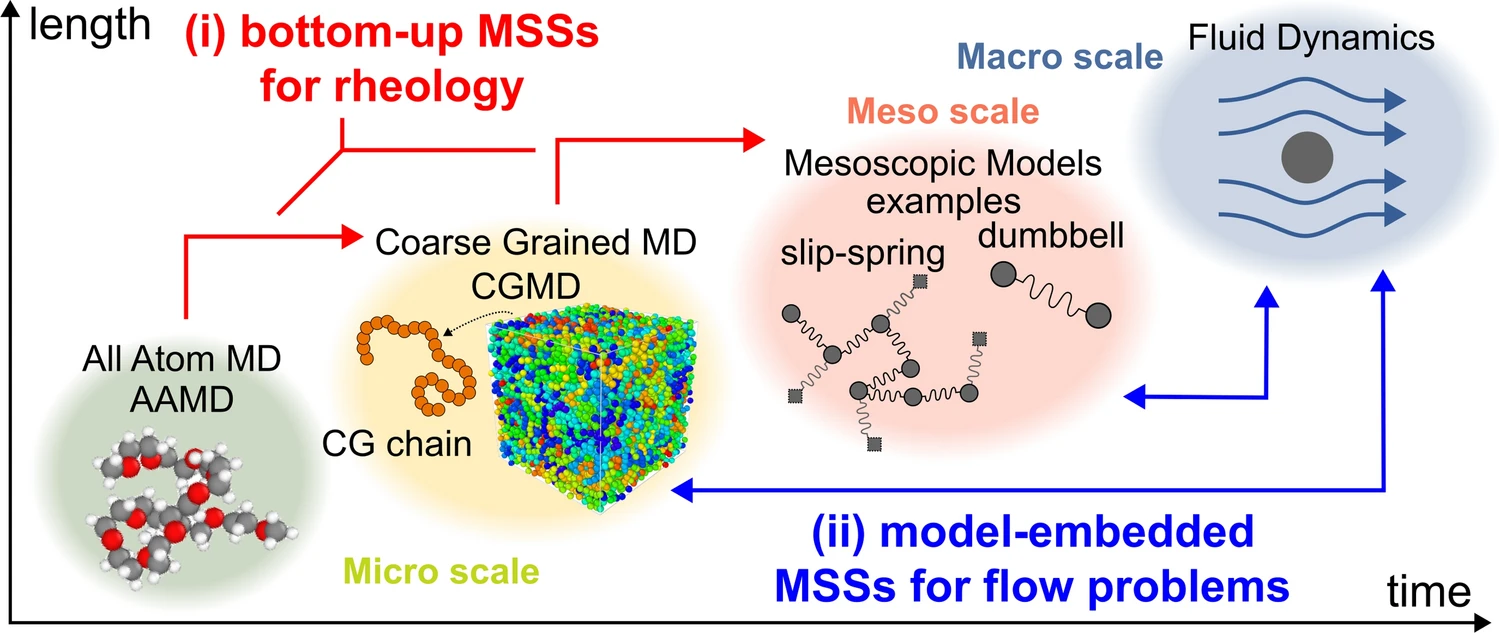
\includegraphics[width=0.8\textwidth]{Fig/duochidumoni.png}
  \FigureBicaption{\label{duochidumoni} 多尺度模拟示意图\cite{satoRecentDevelopmentsMultiscale2024}}{Schematic illustration of Multiscale Simulation\cite{satoRecentDevelopmentsMultiscale2024}}
\end{figure}

传统本构方程的研究方法主要依赖于物理实验和理论推导,通过建立数学方程来描述材料的力学行为。这种方法虽然具有明确的物理意义,但在处理复杂材料或非线性行为时,往往面临模型精度不足、参数识别困难等问题\cite{amamotoDatadrivenApproachesStructureproperty2022}。随着数据驱动技术的快速发展,机器学习为材料本构关系的研究提供了新的思路。通过利用大量实验或仿真数据,机器学习能够自动挖掘材料行为中的潜在规律,构建高精度的预测模型,从而弥补传统方法的不足,并为材料科学的研究开辟了更加智能化的路径。
\section{数据驱动方法流变学本构建模}
\subsection{机器学习方法介绍}
机器学习是人工智能的一个重要分支,其核心是通过算法从数据中自动学习规律,并利用这些规律进行预测或决策。与传统编程不同,机器学习不依赖于明确的规则,而是通过训练数据优化模型参数,从而实现对复杂问题的建模和解决。它在图像识别、自然语言处理、推荐系统等领域取得了显著成果\cite{wang2023scientific}。

监督学习是最常见的机器学习类型,适用于有标签的数据集。常见的算法包括线性回归和逻辑回归,分别用于连续值的预测和二分类问题\cite{uesaka1973theory,liu2021self}。决策树(DT)通过树状结构进行决策,适用于分类和回归任务\cite{quinlan1986induction}。随机森林(RF)是多个决策树的集成,通过投票或平均提高预测准确性\cite{breiman2001random}。支持向量机(SVM)通过寻找最优超平面进行分类,适用于高维数据\cite{cortes1995support}。K近邻算法(KNN)基于距离度量进行分类或回归,简单但计算量大\cite{cover1967nearest}。

随着数据规模和计算能力的提升,深度学习作为机器学习的一个子领域迅速崛起。深度学习通过构建多层的神经网络结构,能够自动提取数据中的多层次特征,从而在处理高维、非线性问题(如图像、语音和文本)时表现出更强的能力,成为推动人工智能发展的核心技术之一\cite{wang2023scientific}。

近年来,深度学习领域在理论创新与应用拓展方面取得了显著进展,极大地推动了机器学习技术的前沿发展。在生成模型领域,扩散模型通过模拟数据从噪声分布到目标分布的逆扩散过程,逐步生成高保真度的图像样本,在图像生成、风格迁移和图像修复等任务中展现出卓越的性能\cite{yang2023diffusion}。在多模态学习方面,研究者通过联合建模文本、图像、音频和视频等多种模态数据,实现了更全面的语义理解与跨模态生成。以模型为代表的多模态预训练框架,通过对比学习策略学习图像-文本对的联合表示空间,在零样本分类和跨模态检索任务中取得了突破性进展\cite{xu2023multimodal}。在自监督学习领域,研究者通过设计预训练任务从数据本身生成监督信号,显著降低了对人工标注数据的依赖\cite{Xie2023}。对比学习作为自监督学习的核心范式之一,通过最大化正样本对的表示一致性并最小化负样本对的相似性,有效提升了模型的特征提取能力\cite{Zhu2024Vision}。这些前沿进展不仅深化了深度学习理论体系,也为解决实际问题提供了新的方法论支持。未来,随着计算能力的提升和数据规模的扩大,深度学习技术有望在医疗影像分析、自动驾驶、智能内容创作等领域展现出更广泛的应用潜力。同时,模型的可解释性、鲁棒性和能效优化等方向仍面临重要挑战,需要跨学科合作以推动该领域的持续发展\cite{wang2023scientific}。

\subsection{机器学习流变学应用研究现状}
\subsubsection{引言}
传统机器学习或是目前最前沿的深度学习研究,最初都集中于计算机科学、人工智能领域,但是近年来在物理学领域,机器学习与物理学问题的研究结合也日益密切\cite{choudhary2022recent}。在量子物理中,机器学习被用于量子态重构、量子电路优化和量子相变识别,显著提高了量子系统的分析和计算效率\cite{biamonte2017quantum}。在凝聚态物理领域,机器学习通过预测材料性质和分类相图,加速了新材料的发现和设计\cite{choudhary2022recent}。在天体物理中,机器学习被用于引力波探测和宇宙微波背景辐射分析,揭示了宇宙的起源和结构\cite{bufano2023machine}。在流体动力学中,机器学习通过数据驱动的方法直接从流体数据中学习湍流动力学,显著提高了湍流模型的精度和计算效率\cite{bruntonMachineLearningFluid2020}。此外,机器学习中的符号回归技术能够从实验数据中自动发现物理定律,为探索未知物理规律提供了新工具\cite{udrescuAIFeynmanPhysicsinspired2020},在多尺度物理系统中,机器学习被用于气候模拟和生物信息学建模,预测复杂动态和处理多重空间和时间尺度的混沌系统。

在流变学领域,机器学习也被广泛应用。传统的流变学研究方法如上一章所述,通过获取数据,通过数学物理方程解释数据。传统的流变学家总是期待于对每个流变学体系建立一个可表示的数学方程,尽管这个方程可能完全无法求出解析解也极难获取稳定精确的数值解。这本质上是一个由因推果的过程,而数据驱动的机器学习方法则从真实的结果出发,构建一个完全匹配的数学方程,这个方程的形式与参数都不确定,但是可以泛化本构现象,即通过含有大量参数的非方程化的计算机模型代替具体形式的本构方程来解决流变学本构问题\cite{colenMachineLearningActivenematic2021,bahiuddinReviewModelingSchemes2024,mangalDatadrivenTechniquesRheology2025}。
\begin{figure}[htbp]
  \centering
  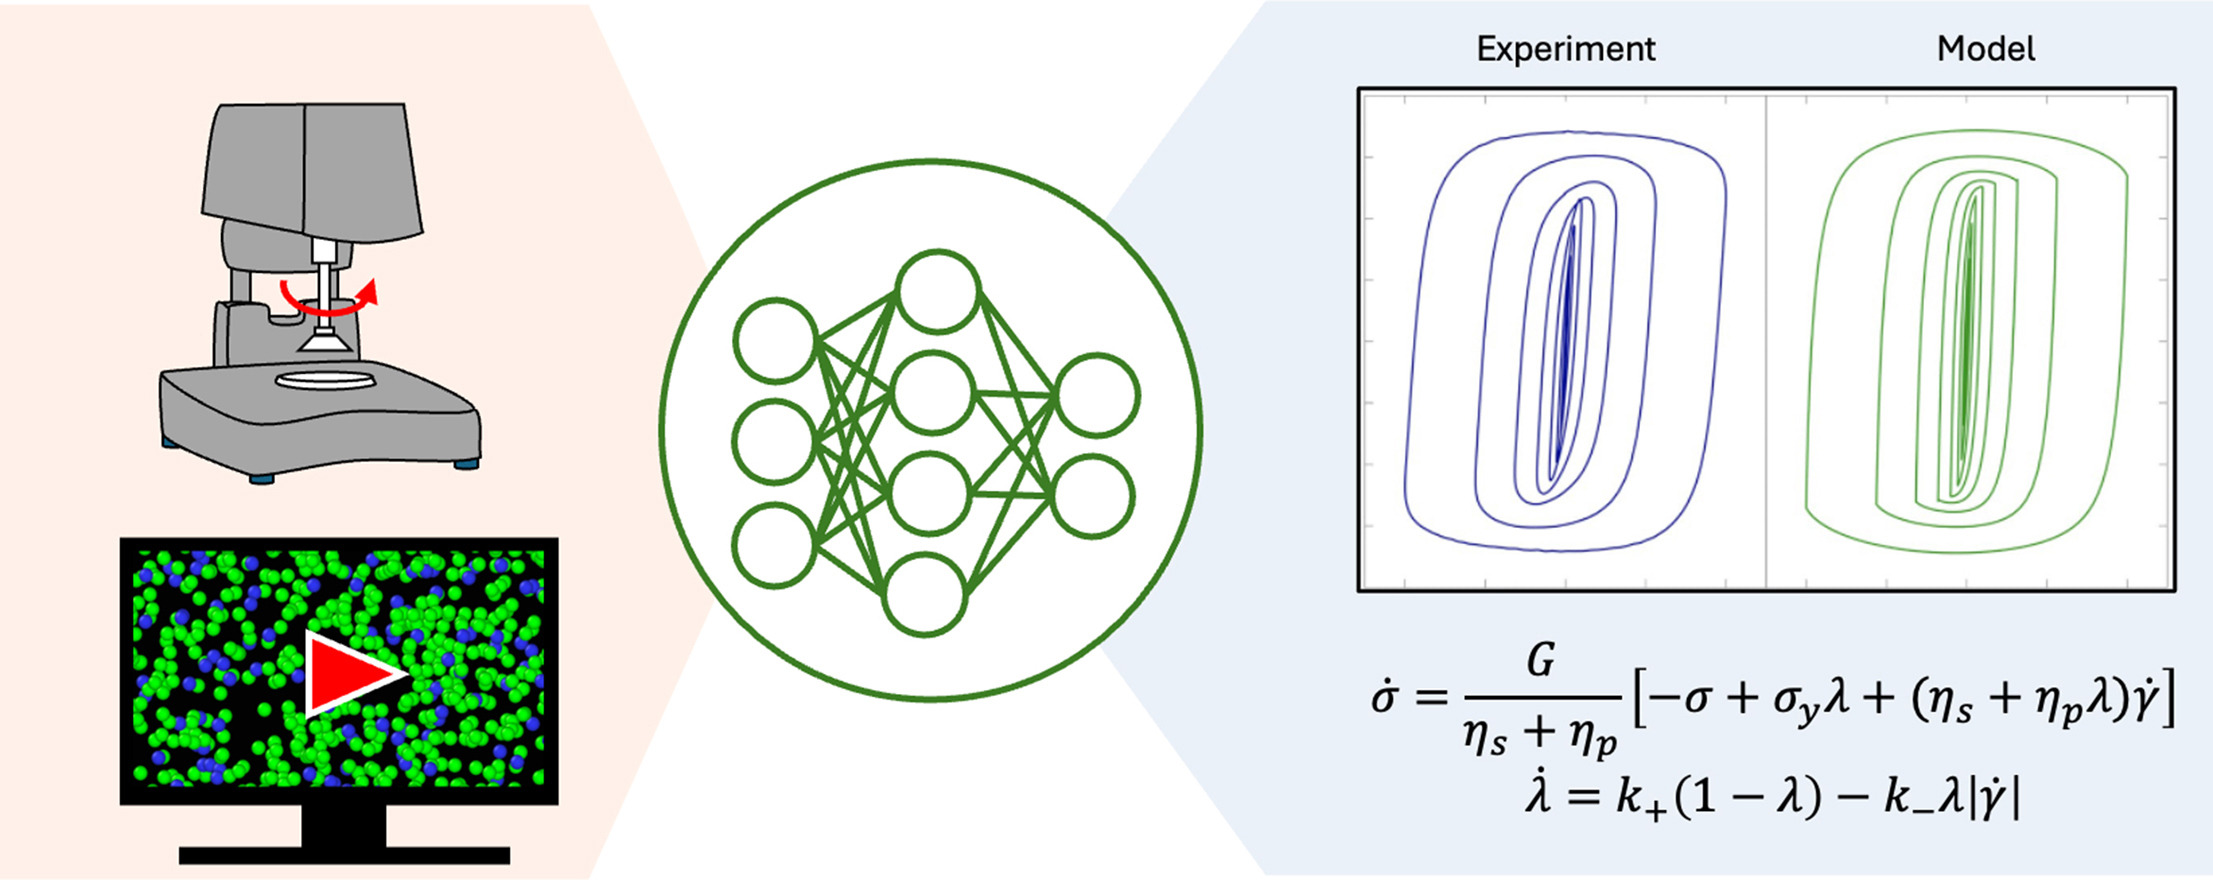
\includegraphics[width=0.8\textwidth]{Fig/datadrivenintro.jpg}
  \FigureBicaption{\label{datadrivenintro} 数据驱动方法应用于流变学研究示意图\cite{mangalDatadrivenTechniquesRheology2025}}{Schematic illustration of data-driven methods applied to rheology research\cite{mangalDatadrivenTechniquesRheology2025}}
\end{figure}

\subsubsection{流变特性预测}
机器学习应用于流变学本构的其中一个应用是流变特性的预测。人工神经网络(ANN)已被用于自动监测合成油基泥浆的各种流变特性,使用泥浆密度和沼泽漏斗作为输入,预测值与实际测量值非常接近,平均绝对误差小于 9.66\%\cite{alsabaaMachineLearningModel2022}。混合机器学习模型结合了ANN和SVM准确预测了纳米基水基钻井液的流变性和过滤特性。四种不同的模型——多元线性回归(MLR)、SVM、回归决策树(CART)和ANN被一起使用,以根据溶液特性预测聚合物溶液的粘度,有助于提高石油采收率\cite{shakeel2023application}。此外,机器学习模型可以与微流体或其他设备集成,用于复杂流体的原位粘度测量。例如,Mustafa等设计了一种微流体传感设备,利用流固耦合和ML算法来测量复杂流体的粘度\cite{mustafaMachineLearningBased2023}。他们采用SVM和KNN算法,分别实现了89.7\%和98.9\%的平均准确率。Ponick等利用卷积神经网络(CNN)通过立体相机图像预测Bingham流体的流变特性\cite{Ponick2022}。Chen等人通过将群贡献(GC)方法与著名的机器学习算法,即人工神经网络 (ANN) 相结合,以预测离子液体 (IL) -水混合物的粘度\cite{CHEN2022118546}。Zhang等人开发了一种深度半监督的基于即时学习的高斯过程回归 (DSSJITGPR) 用于门尼粘度估计\cite{polym14051018}。它将即时学习、半监督学习和深度学习集成到一个统一的建模框架中。DSSJITGPR的有效性和优越性已通过工业橡胶混炼过程的Mooney粘度预测结果得到验证。

\subsubsection{材料表征和工艺设计优化}
机器学习在流变学本构中的应用不仅限于材料表征和工艺设计/优化,还通过直接引入材料制备和表征中的各种参数作为特征,显著简化了传统本构方程中针对特定材料体系拟合不同参数的复杂性。与传统统计方法相比,机器学习算法能够更高效地对这些复杂关系进行建模,其中主成分分析和深度神经网络等技术在管理和减少材料表征中常见的高维数据方面发挥了重要作用,从而实现了更高效的分析和解释。这些方法已广泛应用于3D打印混凝土、纤维增强混凝土、聚合物纳米复合材料、生物墨水、食品材料和高分子科学等领域。Zhang和Shao的研究进一步探讨了基于图像的机器学习技术在材料科学中的应用,以应对各种挑战和任务,由于这些方法的通用性和可转移性,它们同样适用于流变学表征\cite{zhang2022image}。机器学习模型还彻底改变了高通量表征,为数据分析、预测和优化提供了强大的工具。例如,Zhang等人开发了一种自主高通量系统,采用支持向量机(SVM)、随机森林(RF)和极端梯度提升(XGB)分类器等监督式机器学习算法,快速表征水凝胶的流变特性,所有模型在水凝胶相分类中均表现出色\cite{zhangRapidAutonomousHighthroughput2023}。Verheyen等人则利用基于树的集成算法(如随机森林和梯度提升)将数据驱动建模与颗粒水凝胶基质系统的实验优化相结合,这些技术因其在处理分类或回归任务、非线性关系、高维数据和混合数据类型方面的灵活性而被选用\cite{verheyenIntegratedDatadrivenModeling2023}。Martineau等人开发了一种基于高斯过程(GP)建模的管道,用于识别细菌嵌入的丝水凝胶的凝胶化状态,通过比较人类专家和机器学习引导算法的性能,发现两者结合最能加速发现过程\cite{martineauEngineeringGelationKinetics2022}。此外,随机森林和多元线性回归(MLR)等技术已被用作回归工具,将从大振幅振荡剪切(LAOS)实验中获得的流变特性与人类感官感知(如涂抹性)相关联,从而改进化妆品行业的配方设计。Lee等人的研究表明,由于流变测量和铺展性之间的非线性关系,随机森林模型的性能优于多元线性回归模型\cite{lee2022predictive}。

\subsubsection{流变学计算模拟}
机器学习为流变学的计算模拟提供助力,计算平台已经成为流变学研究的重要支柱,广泛应用于从聚合物动力学到颗粒系统的详细模拟,为复杂流体在不同条件下的行为提供了深刻的物理见解。然而,这些技术的主要瓶颈在于模拟与实验条件相关的时间和长度尺度的能力。由于大规模模拟中的大部分计算资源消耗在重复的数学运算上,而这些运算可以通过数据驱动技术高效学习,因此将机器学习与模拟相结合能够显著提升效率和精度。例如,Lu等人基于卷积神经网络的仿真模型在颗粒流模拟中实现了显著的加速,同时保持了较高的精度\cite{lu2021machine}。高斯过程回归则被Seryo等人用于从微观聚合物模拟中推断本构关系,并将这些关系应用于宏观流动仿真,从而调整流体中的应力分布以反映微观动力学\cite{seryoLearningConstitutiveRelation2020}。类似的方法还被应用于缠结良好的聚合物熔体,通过机器学习的本构关系优化模拟效果。此外,Bai等人介绍了一种数据驱动的平滑粒子流体动力学方法,该方法利用实验数据提高了牛顿流体和非牛顿流体的建模精度,即使在数据集较小的情况下也能准确预测幂律流体的速度曲线,同时显著优化计算时间\cite{baiDatadrivenSmoothedParticle2021}。多尺度建模通过在不同尺度之间交换信息来捕捉材料的复杂行为,例如Li等人基于生成对抗网络的方法实现了从粗粒度到原子级别的结构回溯映射\cite{liBackmappingCoarsegrainedMacromolecules2020}。主动学习作为一种高效的机器学习范式,通过选择性地标记信息量最大的数据点,以最少的数据优化学习过程,例如在多尺度建模中,Zhao等人基于高斯过程回归的主动学习策略将所需的模拟次数大幅减少,显著提高了研究复杂材料行为的效率\cite{zhaoActiveLearningConstitutive2018}。这些技术的结合不仅提升了模拟的精度和效率,还为流变学研究提供了更强大的工具。

\subsubsection{小结}
以数据为中心的机器学习模型严重依赖丰富的训练数据来确保预测的可靠性和准确性,无论其架构或算法如何设计。此外,材料特性通常对成分和加工条件的细微变化表现出高度敏感性,这可能导致材料行为的显著变化。因此,数据收集过程必须足够全面和细致,以捕捉这种复杂性,从而确保以数据为中心的模型能够做出准确的预测。例如,对于具有整体Herschel-Bulkley类型行为的屈服应力流体,如果算法仅暴露在大变形率或小变形率下的数据中,它将无法对观察域之外的一般行为做出可靠预测\cite{mangalDatadrivenTechniquesRheology2025,saadatRheologistsGuidelineDatadriven2023,reyesLearningUnknownPhysics2021}。更重要的是,这些模型完全依赖于数据相关性和统计规律,而忽略了基础科学理论的支持,例如黏弹性材料的时间依赖性和应变依赖性等关键物理特性。纯数据驱动方法往往忽视了这些物理细节,导致模型在实际应用中可能失效。因此,在开发算法时,我们应当引入物理约束,将黏弹性的时间依赖性等基本物理规律纳入模型框架,以弥补数据驱动方法的不足,从而提升模型的预测能力和泛化性能。
\section{引入物理约束的神经网络研究}
\subsection{引言}
近年来,多种方法被提出并广泛应用于将基本物理规则和领域知识整合到机器学习框架中,这些方法在众多领域展现了深远的影响。这类模型的总体框架通常被称为物理信息机器学习(PIML)。PIML的一个开创性范例是“物理信息神经网络”(PINN),它代表了科学计算和应用数学领域的重大突破\cite{karniadakisPhysicsinformedMachineLearning2021,raissiPhysicsinformedNeuralNetworks2019}。PINN将机器学习算法与从系统观察、经验以及物理或数学理解中获得的先验知识无缝结合,通过将这些先验知识直接嵌入模型架构中,显著减少了对大规模训练数据集的依赖,从而能够利用更少的观测数据解决复杂的物理问题。

\subsection{物理信息神经网络研究现状}
近年来,物理信息神经网络(PINN)在流变学建模领域取得了重要进展,有效克服了传统方法依赖简化假设和难以处理复杂材料特性的局限。Mahmoudabadbozchelou等人提出的流变学信息神经网络(RhINN)框架,能够处理触变性弹性粘塑性(TEVP)模型等多种本构模型\cite{mahmoudabadbozchelouRheologyInformedNeuralNetworks2021}。该框架以时间t和剪切速率为输入,剪应力$\sigma$和结构参数$\lambda$为输出,通过最小化包含方程残差和初始条件差异的损失函数来训练网络参数。在逆问题求解中,RhINN可同时学习网络参数和流变参数,其预测结果与真实数据高度吻合,展现了良好的鲁棒性。Dabiri等人进一步将RhINN扩展至分数阶微分方程,提升了其在复杂本构模型参数识别中的应用价值\cite{dabiri2023}。在相关研究中,Zhang等人开发的RheologyNet成功应用于胶凝材料触变特性评估,其预测结果与有限元分析高度一致\cite{zhangRheologyNetPhysicsinformedNeural2023}。Nagrani等人则利用PINN研究了导热硅脂的流变行为,通过实验数据确定了流变参数\cite{nagrani2023}。基于物理的机器学习方法还可从间接观测中学习未知流变模型,例如通过三维流场数据推断广义牛顿流体的稳态剪切粘度,这一方法在聚合物熔体和颗粒悬浮液研究中取得了显著成果。此外,PINN在稀薄气体流动预测中也展现出应用潜力\cite{tucnyLearningViscosityFunctions2024}。Howard等人将悬浮平衡模型与神经网络结合,成功预测了单分散悬浮液的颗粒应力,但在双分散系统中的应用仍存在局限。这些研究充分展示了物理信息神经网络在流变学领域的广泛应用前景\cite{howardMachineLearningMethods2023}。
\begin{figure}[htbp]
  \centering
  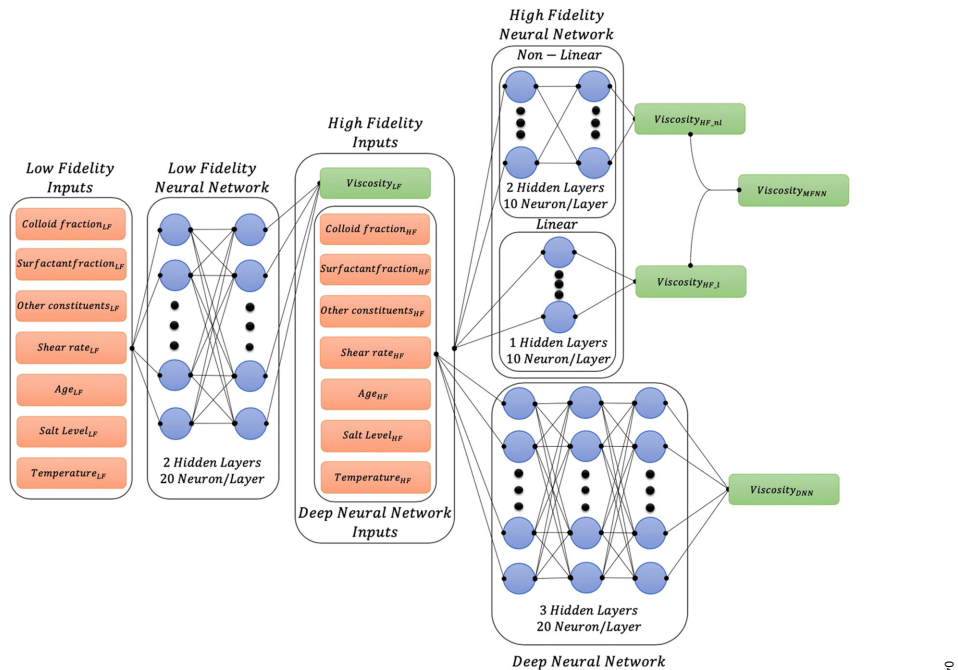
\includegraphics[width=0.8\textwidth]{Fig/MFNN.png}
  \FigureBicaption{\label{mdnn} 多保真神经网络(MFNN)结构示意图\cite{mahmoudabadbozchelouDatadrivenPhysicsinformedConstitutive2021}}{ Schematic illustration of Multifidelity Neural Network (MFNN) structure\cite{mahmoudabadbozchelouDatadrivenPhysicsinformedConstitutive2021}}
\end{figure}

多保真度建模是一种强大的技术,通过整合来自不同保真度和计算成本的数据来增强模型预测能力。这种方法在物理定律不精确或高保真数据生成成本较高的情况下尤为有用。通过高效结合高保真和低保真数据,多保真度建模为复杂系统的精确建模提供了一种更高效且更具成本效益的解决方案。例如,Mahmoudabadbozchelou等人利用多保真度方法构建了一个流变学元模型,用于预测复杂多组分系统的流变响应,同时考虑了老化、混合物的盐度和温度依赖性等输入参数\cite{mahmoudabadbozchelouDatadrivenPhysicsinformedConstitutive2021}。在该框架中,低保真数据通过多种本构方程生成,而高保真数据则来自实验测量。与传统的高保真神经网络相比,这种组合方法显著提高了预测精度,充分展示了多保真度建模的优势。

类似的方法也被应用于预测纤维悬浮液的流变特性,其中基于法向载荷相关摩擦系数模型的数值模拟用于生成高保真数据,而低保真数据则通过不同的本构模型生成。纤维的物理特性,包括纵横比、纤维刚度、表面粗糙度以及体积分数,均被用作输入参数。这种将基础物理特性融入机器学习算法的模式并不局限于特定方法,因此多保真度建模也可以与直接或反向流变学信息神经网络(RhINN)相结合,以利用不同级别的数据准确性来优化模型预测。这种混合方法能够从有限的实验观察中做出高度准确的流变学预测,例如Mahmoudabadbozchelou等人对气相硅胶流变学的成功预测\cite{mahmoudabadbozchelouDigitalRheometerTwins2022}。虽然多保真度算法通常依赖于不同准确性数据的可用性,但在上述应用中,这些数据是通过描述目标系统的物理或现象学模型直接生成的,因此这些方法被归类为物理信息建模。然而,如果不同保真度级别的数据源与基础物理学无关,则该方法更倾向于以数据为中心。例如,分层机器学习模型通过结合墨水和打印机参数之间的已知物理关系,能够在小数据集上实现精确建模。这种灵活性使得多保真度建模在流变学和其他复杂系统的研究中具有广泛的应用潜力。
\begin{figure}[htbp]
  \centering
  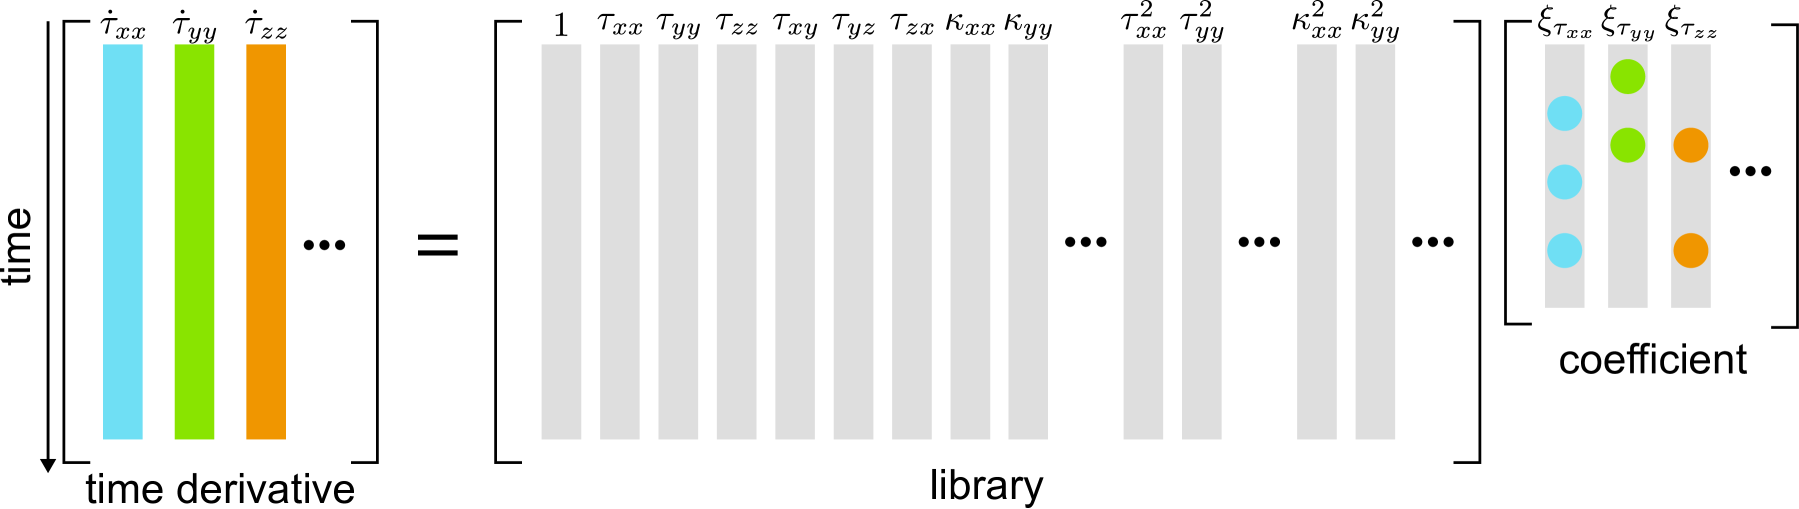
\includegraphics[width=0.8\textwidth]{Fig/xianxingxishu.png}
  \FigureBicaption{\label{xianxingxishu} Rheo-SINDy的示意图\cite{Sato2025}}{Schematic illustration of Rheo-SINDy\cite{Sato2025}}
\end{figure}
\begin{figure}[htbp]
  \centering
  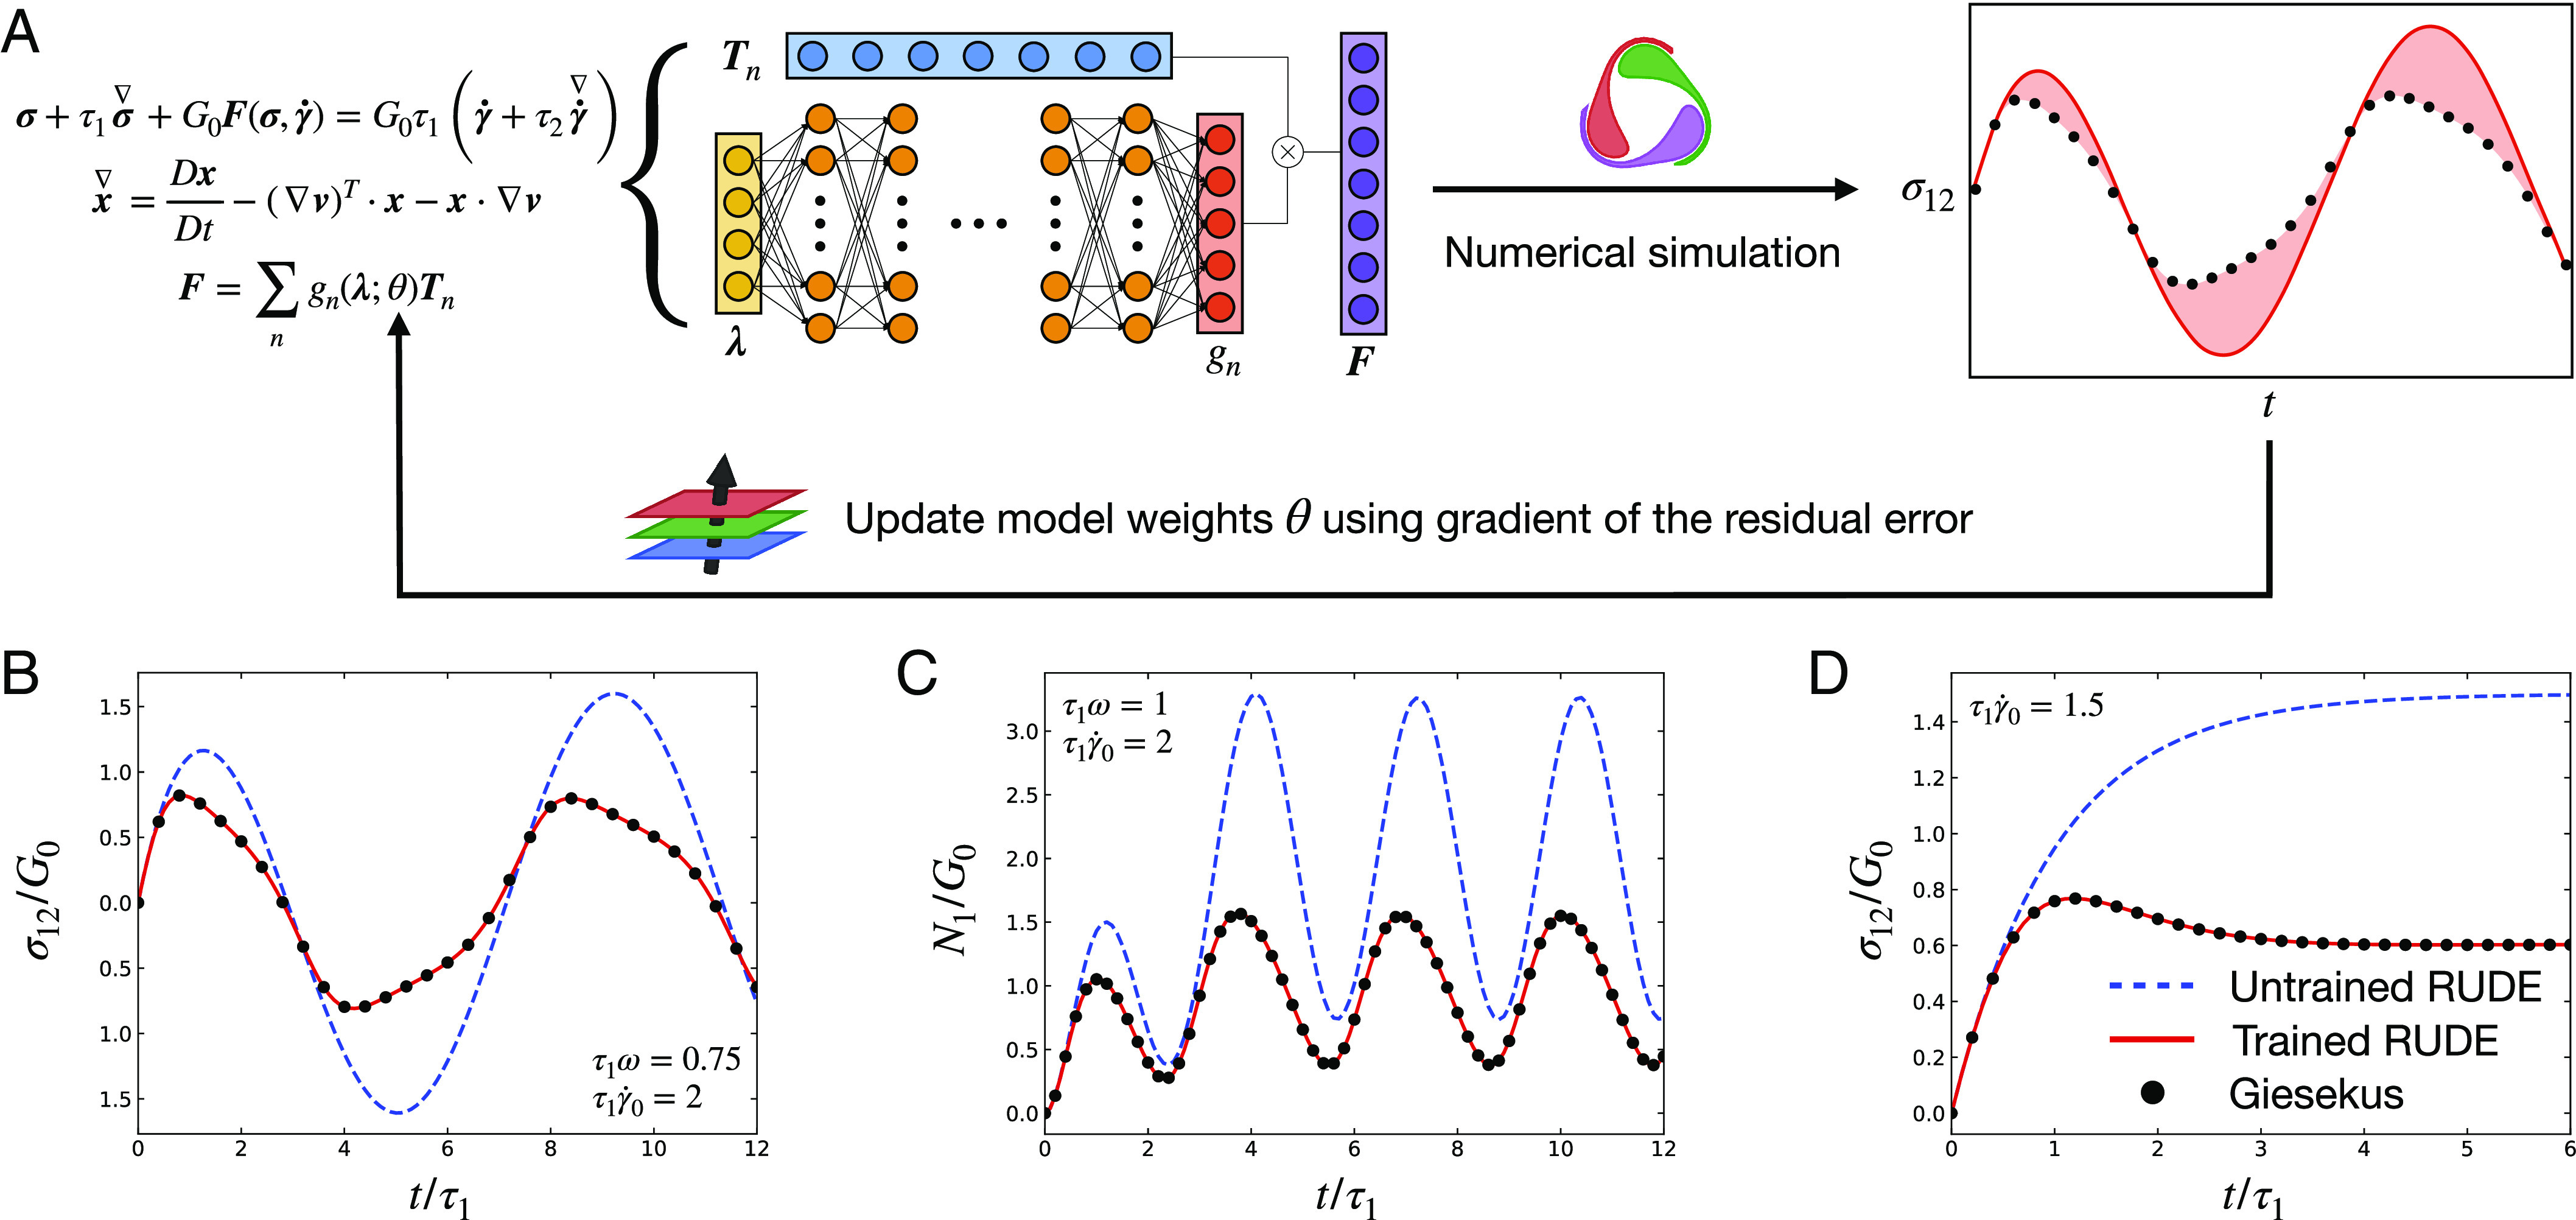
\includegraphics[width=0.8\textwidth]{Fig/pnas.2304669120fig01.jpg}
  \FigureBicaption{\label{lennon} (A) RUDE 训练循环示意图(B–D)基于Giesekus模型合成LAOS数据训练的RUDE评估结果,黑色圆圈:测试数据;红色线条:训练后的RUDE;蓝色线条:未训练的 RUDE(B) 中间频率下的剪切应力响应(C) 训练频率下的法向应力(D) 稳态剪切流启动时的剪切应力响应\cite{lennonScientificMachineLearning2023a}}{(A) Schematic depiction of a RUDE within the training loop (B–D) Evaluation of a RUDE trained on synthetic LAOS data for the Giesekus model,Black circles: test data; red lines: trained RUDE; blue lines: untrained RUDE (B) Shear stress response at an intermediate frequency (C) Normal stress at a training frequency (D) Shear stress during startup of steady shear flow\cite{lennonScientificMachineLearning2023a}}
\end{figure}
机器学习技术的另一个重要应用在于发现闭式本构关系,这些关系从数学上描述了应力和变形之间的关联。这一过程通常通过分析实验数据并结合非线性动力学稀疏识别(SINDy)和符号回归等技术来实现\cite{Sato2025}。在这些方法中,通常采用多步骤流程:首先从广泛的潜在函数列表中筛选出最重要的候选函数,然后精确恢复这些函数的参数,以最简洁的形式描述动力学系统。例如,SINDy方法被直接扩展到流变学应用中,开发了一种称为Rheo-SINDy的稀疏识别方法,用于从已知方程库生成的流变学数据中恢复本构方程。然而,现有方法在处理不完整、稀缺或噪声数据时面临挑战,特别是需要数值微分来计算导数以构建控制方程\cite{mahmoudabadbozchelouUnbiasedConstructionConstitutive2024}。这一问题可以通过结合自动微分功能的物理信息神经网络(PINN)来解决,从而避免数值微分的需求。这种组合方法被称为PINN-SR(具有稀疏回归的PINN),已成功应用于从模型弹性粘塑性流体的实验数据中提取精确的本构关系。

尽管目前大多数机器学习技术(无论是数据驱动还是物理信息)都集中在单个标量分量(如剪切应力、微观结构参数或粘度)作为流变学特征,并与粘度流动和体材料函数预测相关,但真正可推广的流变学机器学习技术必须具备张量性质,并避免客观性问题。Lennon等人提出的RUDE框架优雅地解决了这些基本约束,构建了包含物理信息的可学习模型,同时对特定实验协议或流动运动学的细节保持不可知\cite{lennonScientificMachineLearning2023a}。在该框架中,广义粘弹性模型中的未知非线性项被表示为张量基函数的线性组合,这些函数强制执行对称性和框架不变性等物理约束,而张量基函数的系数则通过神经网络输出建模。RUDE框架的一个显著优势在于,其预测不仅能够推广到观测域之外,还可以扩展到应力张量的其他分量,从而实现完全解析的流动预测。这种能力使得RUDE在流变学应用中展现出强大的泛化能力和实用性。
\subsection{其他物理信息深度学习模型}
近年来,深度神经算子作为一种新的机器学习模型被提出,用于隐式学习物理现象的解算子\cite{luLearningNonlinearOperators2021}。与使用有限维向量空间的标准神经网络不同,神经算子学习函数空间之间的映射。典型的架构包括DeepONet和傅里叶神经算子(FNO)及其变体。DeepONet由两个子网络组成:分支网络和中继网络,分别提取输入函数和输入坐标的潜在表示,并通过点积合并输出。FNO通过在傅里叶空间中参数化积分核来实现高效的架构。神经算子可以作为隐藏控制方程的隐式解算子,使其成为理解复杂物理系统的强大工具。它们可以与物理场和其他域约束结合,以获得高保真解和良好的泛化能力。

神经算子在简洁且准确地学习复杂动力学方面表现出色,已在流体力学应用中得到验证,如天气预报和碳捕获的储层工程。然而,在复杂流体领域的应用仍有限。Rashid等人采用FNO架构预测了数字复合材料中的应力和应变场\cite{rashid2022learning}。FNO的扩展,如隐式傅里叶神经算子(IFNO),已被证明可以预测不可见载荷条件下的材料响应,并且同样适用于流变学应用\cite{you2022learning}。在IFNO中,层之间的增量由积分算子建模,因此所得架构可以解释为未知控制定律的定点方法。与传统的本构模型相比,这种方法将预测误差减少了十倍。Howard等人还应用了模型算子回归(MOR-physics)框架,从单分散和双分散悬浮液中的体积分数和速度测量中学习粒子应力\cite{howardMachineLearningMethods2023}。

\section{本课题研究介绍}
\subsection{研究内容}
本文旨在通过多方法融合的系统性研究,探索深度学习在模拟数据和实验数据下本构方程的建模与评估,文章主要结构如下,研究路线如图\ref{HolisticResearchFramework}所示。

第一章首先综述了流变学研究的基本问题和应用方向。其次讨论了本构方程理论的发展,经典本构方程的发展历史,数学形式,适用范围等。然后综述了本构方程的研究方法,包括传统的数值方法和近年来被广泛研究的数据驱动机器学习方法。最后综述了将物理约束引入机器学习方法的研究现状,并简述了本文后续的课题设计方案。

第二章主要介绍了本文课题中主要使用的各类算法,从算法理论到选型依据做了综述讨论。
\begin{figure}[htbp]
  \centering
  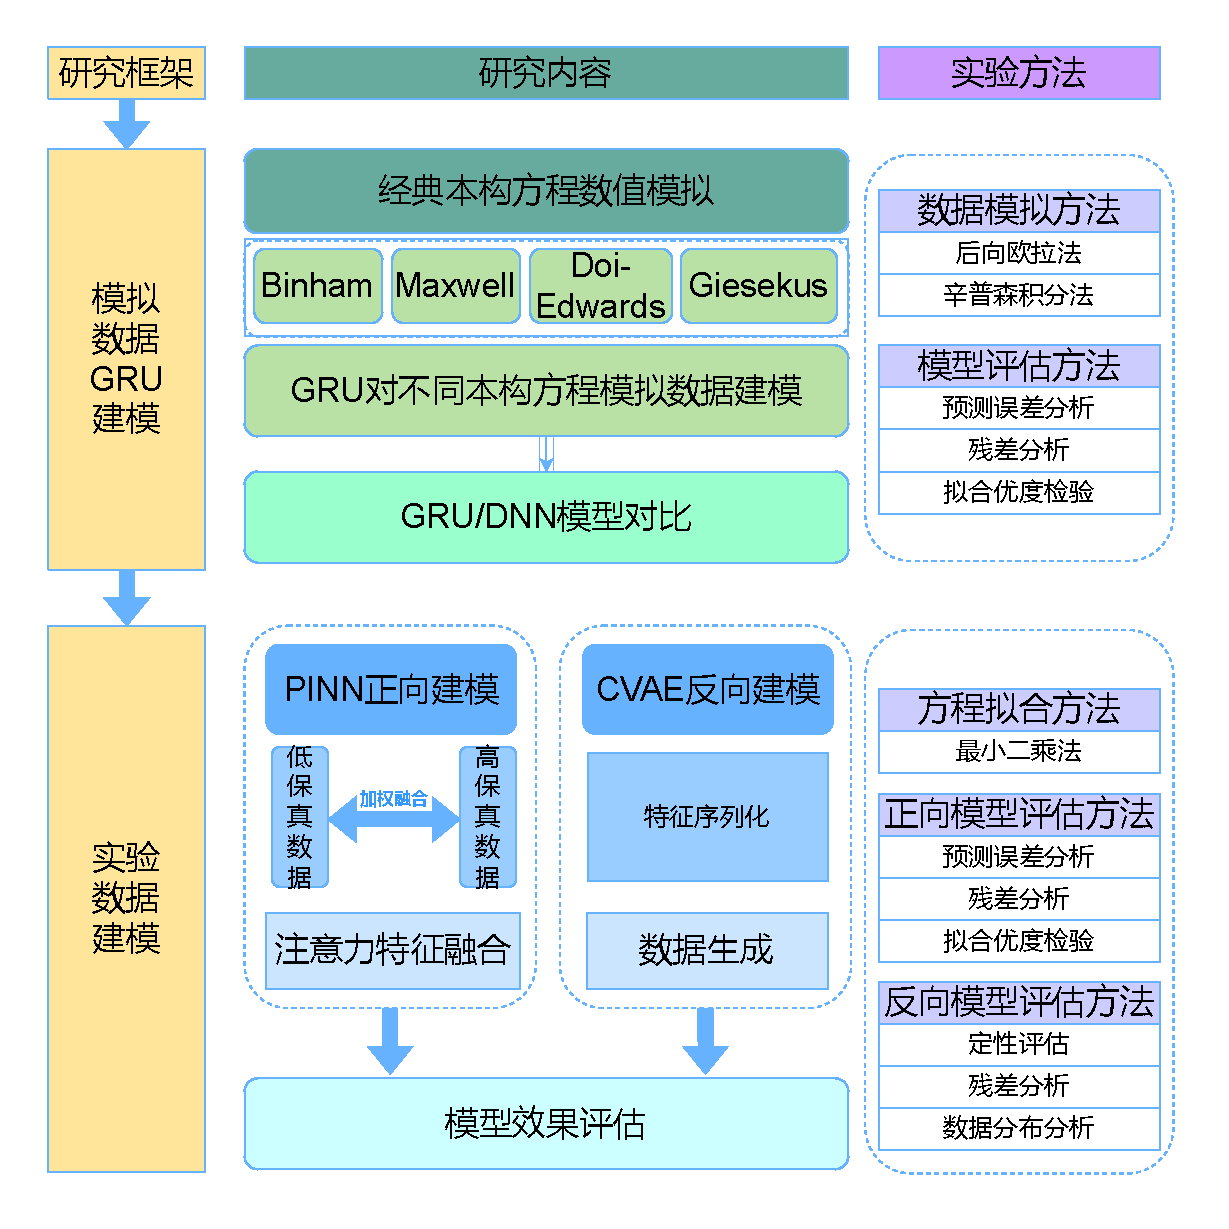
\includegraphics[width=0.8\textwidth]{Fig/HolisticResearchFramework.drawio.pdf}
  \FigureBicaption{\label{HolisticResearchFramework} 研究路线图}{Research roadmap}
\end{figure}
第三章介绍了本文的第一部分工作,使用门控循环单元(GRU)对经典本构方程的模拟数据进行深度学习建模,并使用各种指标对模型性能进行评估。具体来说,首先基于经典本构方程(Binham模型、Maxwell模型、Doi-Edwards模型、Giesekus模型),采用后向欧拉法和辛普森积分法等数值模拟方法生成模拟数据,并划分训练集、验证集、测试集。随后使用GRU分别对不同的模型模拟数据进行建模,训练后使用测试集进行模型的评估,采用决定系数(R$^2$)、平均绝对误差(MAE)、平均绝对百分比误差(MAPE)
等指标,对模型性能进行定量评估。同时在相同的数据集上使用普通深度神经网络(DNN)进行训练,将两套模型进行比较,以验证GRU模型在处理复杂非线性时间依赖性流变学本构方程时的优势。

第四章介绍了本文的第二部分工作,针对黏弹性凝胶材料的真实实验流变数据进行物理信息神经网络(PINN)的建模,在Mahmoudabadbozchelou等人的模型基础之上,进一步优化PINN的模型,采用可学习的损失权重进行损失函数的优化,探究PINN对特定参数下凝胶材料模量及损耗因子的预测能力。随后,采用条件变分自编码器(CVAE)反向建立生成式模型,通过这个模型生成特定流变学数据下的制备参数,并进行生成效果评估。

\subsection{研究创新点}
\begin{enumerate}[topsep = 0 pt, itemsep= 0 pt, parsep=0pt, partopsep=0pt, leftmargin=44pt, itemindent=0pt, labelsep=6pt, label=(\arabic*)]
  \item 本文采用门控循环单元(GRU),通过其门控机制捕捉时间序列数据中的时间依赖性,使模型更贴近复杂流体的物理特性。
  \item 优化Mahmoudabadbozchelou提出的物理信息神经网络(PINN),引入可学习的权重损失以缓解多损失函数的梯度消失问题,并结合注意力特征融合解决实验数据稀疏问题。
  \item 使用CVAE反向建模,以流变学特性反预测制备参数,辅助实验设计。
\end{enumerate}
\subsection{研究意义}
传统机器学习方法在流变学建模中往往局限于单点预测,难以捕捉复杂流体的时间依赖性,而本文采用门控循环单元(GRU)进行建模,充分利用其时间序列处理能力,使模型更贴近黏弹性材料的流变学特性。这一研究不仅拓展了深度学习在流变学领域的应用范围,还为复杂流体建模提供了新的理论支持。随着计算机科学的发展,自注意力机制(如Transformer)在自然语言处理等领域展现了强大的长程依赖捕捉能力。尽管受限于流变学数据的稀缺性,本文未直接采用Transformer架构,但通过探索能够解决长期序列依赖的模型,为未来本构方程建模的研究指明了方向。这一思路有望进一步推动流变学本构建模的发展,为解决复杂流体建模问题提供更强大的工具。

本文通过优化物理信息神经网络(PINN),引入可学习权重和注意力特征融合,为小样本学习提供了新的解决方案,提升了模型在数据稀缺情况下的性能。同时,利用条件变分自编码器(CVAE)进行反向建模,以流变学特性反推制备参数,为实验设计提供了理论支持。这些研究不仅推动了流变学建模方法的进步,还为材料科学和工程领域的实验优化提供了新的思路,具有一定的理论意义和实践价值。